\documentclass[11pt,a4paper]{article}
\usepackage[margin=1in]{geometry}
\usepackage[T1]{fontenc}
\usepackage[utf8]{inputenc}
\usepackage{graphicx}
\usepackage{booktabs}
\usepackage{float}
\usepackage{tabularx}
\usepackage{array}
\usepackage{hyperref}
\usepackage{xcolor}
\hypersetup{colorlinks=true,linkcolor=blue,urlcolor=blue}

\title{SEM Dendrite Segmentation: Comparative Technical Report}
\author{Automated Report Generator}
\date{\today}

\begin{document}
\maketitle

\section*{Abstract}
This report summarizes pixel-level semantic segmentation of lithium dendrites in SEM images using two pipelines:
(1) a deterministic classic morphology pipeline and
(2) a YOLO segmentation model.
The evaluation set includes 10 labeled images.
Average Dice scores are Classic=0.925 and YOLO=0.000.
The report includes quantitative metrics, method comparison tables, and visual success/failure analysis.

\section*{Methodology}
\textbf{Classic Pipeline:} pre-processing (normalization, CLAHE, bilateral denoising), threshold-based segmentation,
morphological cleaning/reconstruction, branch separation, and skeleton extraction.\\
\textbf{Deep Learning Pipeline:} transfer-learned YOLO segmentation model with binary mask output per image.\\
\textbf{Evaluation Metrics:} Dice, IoU, Precision, Recall measured against manual ground-truth masks.

\section*{Results and Discussion}
\subsection*{Average Metrics}
\begin{table}[H]
\centering
\begin{tabular}{lcccc}
\toprule
Method & Dice & IoU & Precision & Recall \\
\midrule
Classic & 0.925 & 0.860 & 0.877 & 0.979 \\
YOLO & 0.000 & 0.000 & 1.000 & 0.000 \\
\bottomrule
\end{tabular}
\caption{Average segmentation metrics across available predictions.}
\end{table}

\subsection*{Per-Image Comparison}
\begin{table}[H]
\centering
\scriptsize
\begin{tabular}{lcccccccc}
\toprule
Image & C-Dice & C-IoU & C-Prec & C-Rec & Y-Dice & Y-IoU & Y-Prec & Y-Rec \\
\midrule
easy\_1 & 0.942 & 0.891 & 0.903 & 0.985 & 0.000 & 0.000 & 1.000 & 0.000 \\

easy\_10 & 0.925 & 0.860 & 0.886 & 0.967 & 0.000 & 0.000 & 1.000 & 0.000 \\

easy\_2 & 0.930 & 0.869 & 0.905 & 0.956 & 0.000 & 0.000 & 1.000 & 0.000 \\

easy\_3 & 0.948 & 0.901 & 0.922 & 0.975 & 0.000 & 0.000 & 1.000 & 0.000 \\

easy\_4 & 0.899 & 0.817 & 0.822 & 0.992 & 0.000 & 0.000 & 1.000 & 0.000 \\

easy\_5 & 0.917 & 0.846 & 0.853 & 0.991 & 0.000 & 0.000 & 1.000 & 0.000 \\

easy\_6 & 0.917 & 0.847 & 0.855 & 0.989 & 0.000 & 0.000 & 1.000 & 0.000 \\

easy\_7 & 0.926 & 0.862 & 0.882 & 0.974 & 0.000 & 0.000 & 1.000 & 0.000 \\

easy\_8 & 0.909 & 0.833 & 0.840 & 0.990 & 0.000 & 0.000 & 1.000 & 0.000 \\

easy\_9 & 0.934 & 0.876 & 0.897 & 0.975 & 0.000 & 0.000 & 1.000 & 0.000 \\
\bottomrule
\end{tabular}
\caption{Per-image metric comparison (first 10 rows). Full table is exported to CSV.}
\end{table}

\subsection*{Failure Analysis}
Number of failures under Dice threshold: 10.
\begin{table}[H]
\centering
\scriptsize
\begin{tabularx}{\linewidth}{llcccX}
\toprule
Image & Method & Dice & Precision & Recall & Estimated Cause \\
\midrule
easy\_1 & YOLO & 0.000 & 1.000 & 0.000 & Under-segmentation - thin branches missed (Classic succeeds -> likely OOD sample for YOLO) \\

easy\_10 & YOLO & 0.000 & 1.000 & 0.000 & Under-segmentation - thin branches missed (Classic succeeds -> likely OOD sample for YOLO) \\

easy\_2 & YOLO & 0.000 & 1.000 & 0.000 & Under-segmentation - thin branches missed (Classic succeeds -> likely OOD sample for YOLO) \\

easy\_3 & YOLO & 0.000 & 1.000 & 0.000 & Under-segmentation - thin branches missed (Classic succeeds -> likely OOD sample for YOLO) \\

easy\_4 & YOLO & 0.000 & 1.000 & 0.000 & Under-segmentation - thin branches missed (Classic succeeds -> likely OOD sample for YOLO) \\

easy\_5 & YOLO & 0.000 & 1.000 & 0.000 & Under-segmentation - thin branches missed (Classic succeeds -> likely OOD sample for YOLO) \\

easy\_6 & YOLO & 0.000 & 1.000 & 0.000 & Under-segmentation - thin branches missed (Classic succeeds -> likely OOD sample for YOLO) \\

easy\_7 & YOLO & 0.000 & 1.000 & 0.000 & Under-segmentation - thin branches missed (Classic succeeds -> likely OOD sample for YOLO) \\

easy\_8 & YOLO & 0.000 & 1.000 & 0.000 & Under-segmentation - thin branches missed (Classic succeeds -> likely OOD sample for YOLO) \\

easy\_9 & YOLO & 0.000 & 1.000 & 0.000 & Under-segmentation - thin branches missed (Classic succeeds -> likely OOD sample for YOLO) \\
\bottomrule
\end{tabularx}
\caption{Failure characterization based on precision/recall patterns.}
\end{table}

\subsection*{Visual Analysis (Successes and Failures)}
\begin{figure}[H]
\centering
\includegraphics[width=0.96\linewidth]{assets/cases/easy_3_analysis.png}
\caption{Success case: easy\_3 (combined Dice=0.474)}
\end{figure}

\begin{figure}[H]
\centering
\includegraphics[width=0.96\linewidth]{assets/cases/easy_9_analysis.png}
\caption{Success case: easy\_9 (combined Dice=0.467)}
\end{figure}

\begin{figure}[H]
\centering
\includegraphics[width=0.96\linewidth]{assets/cases/easy_7_analysis.png}
\caption{Success case: easy\_7 (combined Dice=0.463)}
\end{figure}

\begin{figure}[H]
\centering
\includegraphics[width=0.96\linewidth]{assets/cases/easy_1_analysis.png}
\caption{Failure case: easy\_1 (combined Dice=0.471)}
\end{figure}

\begin{figure}[H]
\centering
\includegraphics[width=0.96\linewidth]{assets/cases/easy_10_analysis.png}
\caption{Failure case: easy\_10 (combined Dice=0.463)}
\end{figure}

\begin{figure}[H]
\centering
\includegraphics[width=0.96\linewidth]{assets/cases/easy_2_analysis.png}
\caption{Failure case: easy\_2 (combined Dice=0.465)}
\end{figure}

\subsection*{YOLO Training Diagnostics}
\begin{figure}[H]
\centering
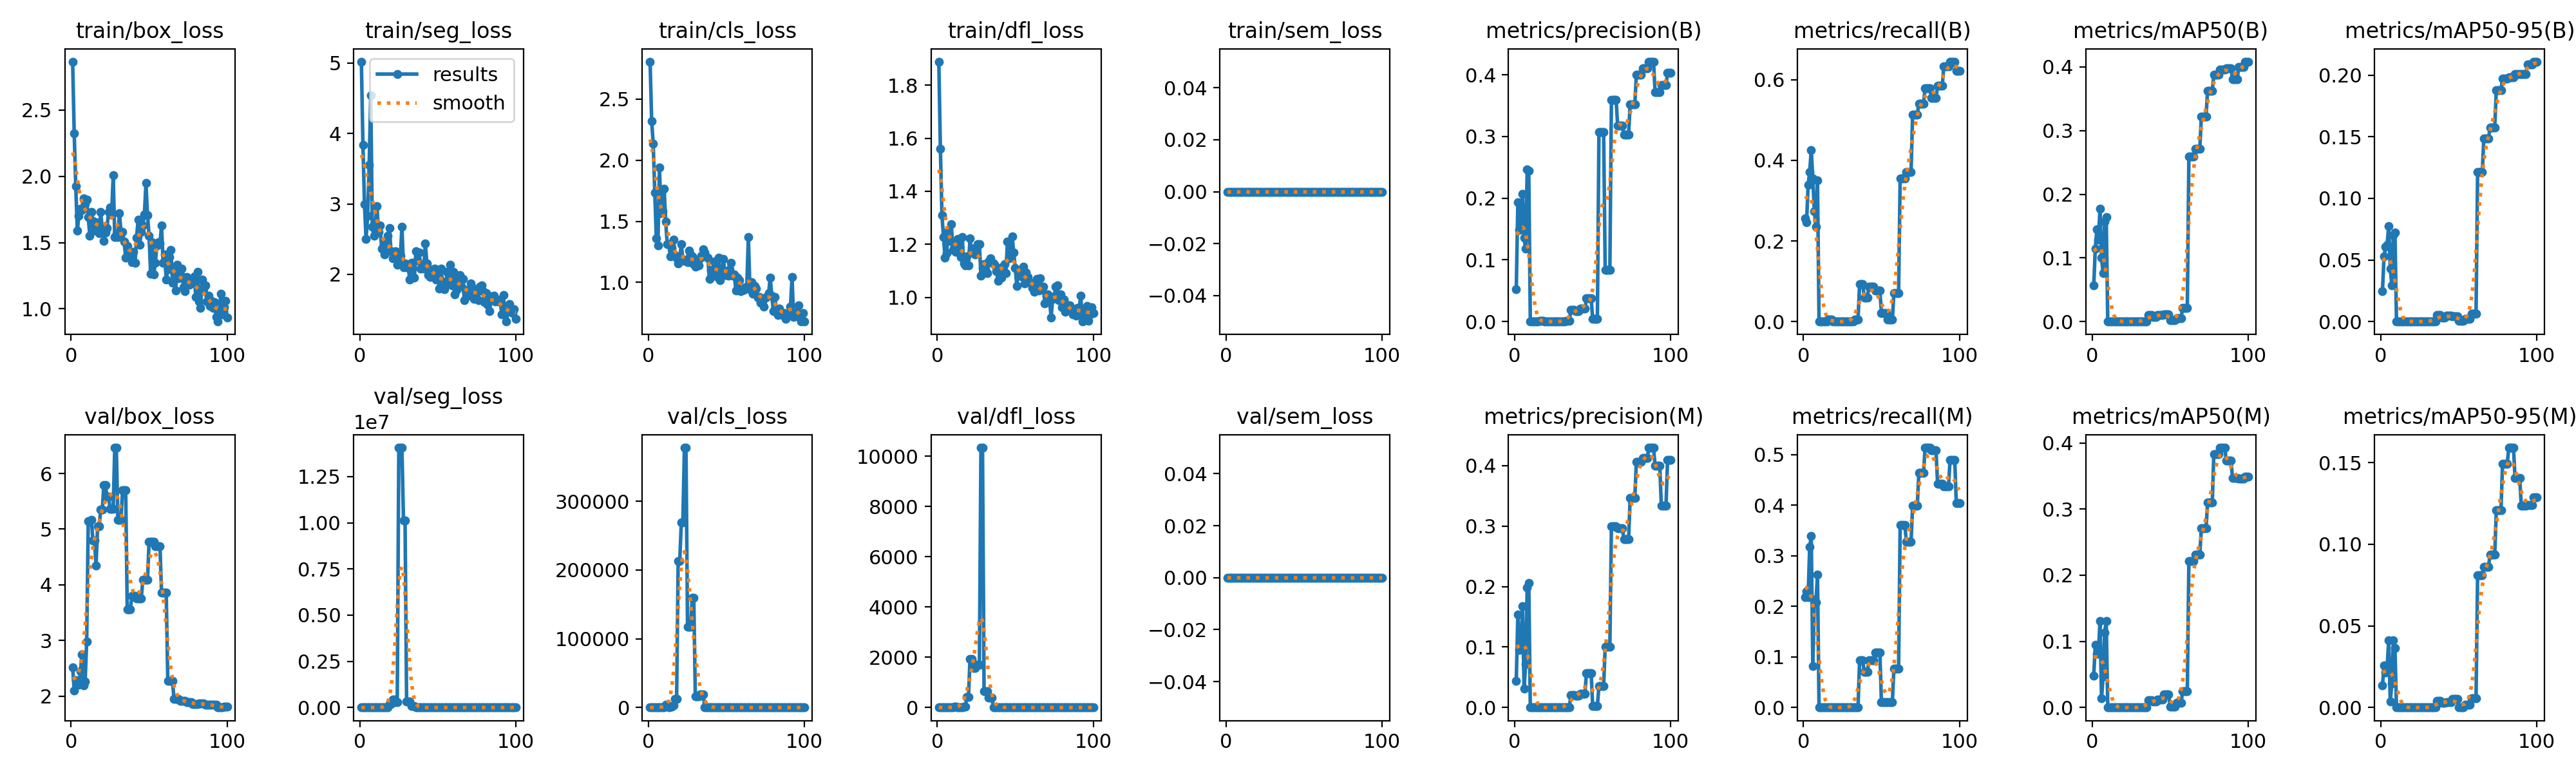
\includegraphics[width=0.92\linewidth]{assets/training/results.png}
\caption{YOLO training metrics over epochs}
\end{figure}

\begin{figure}[H]
\centering
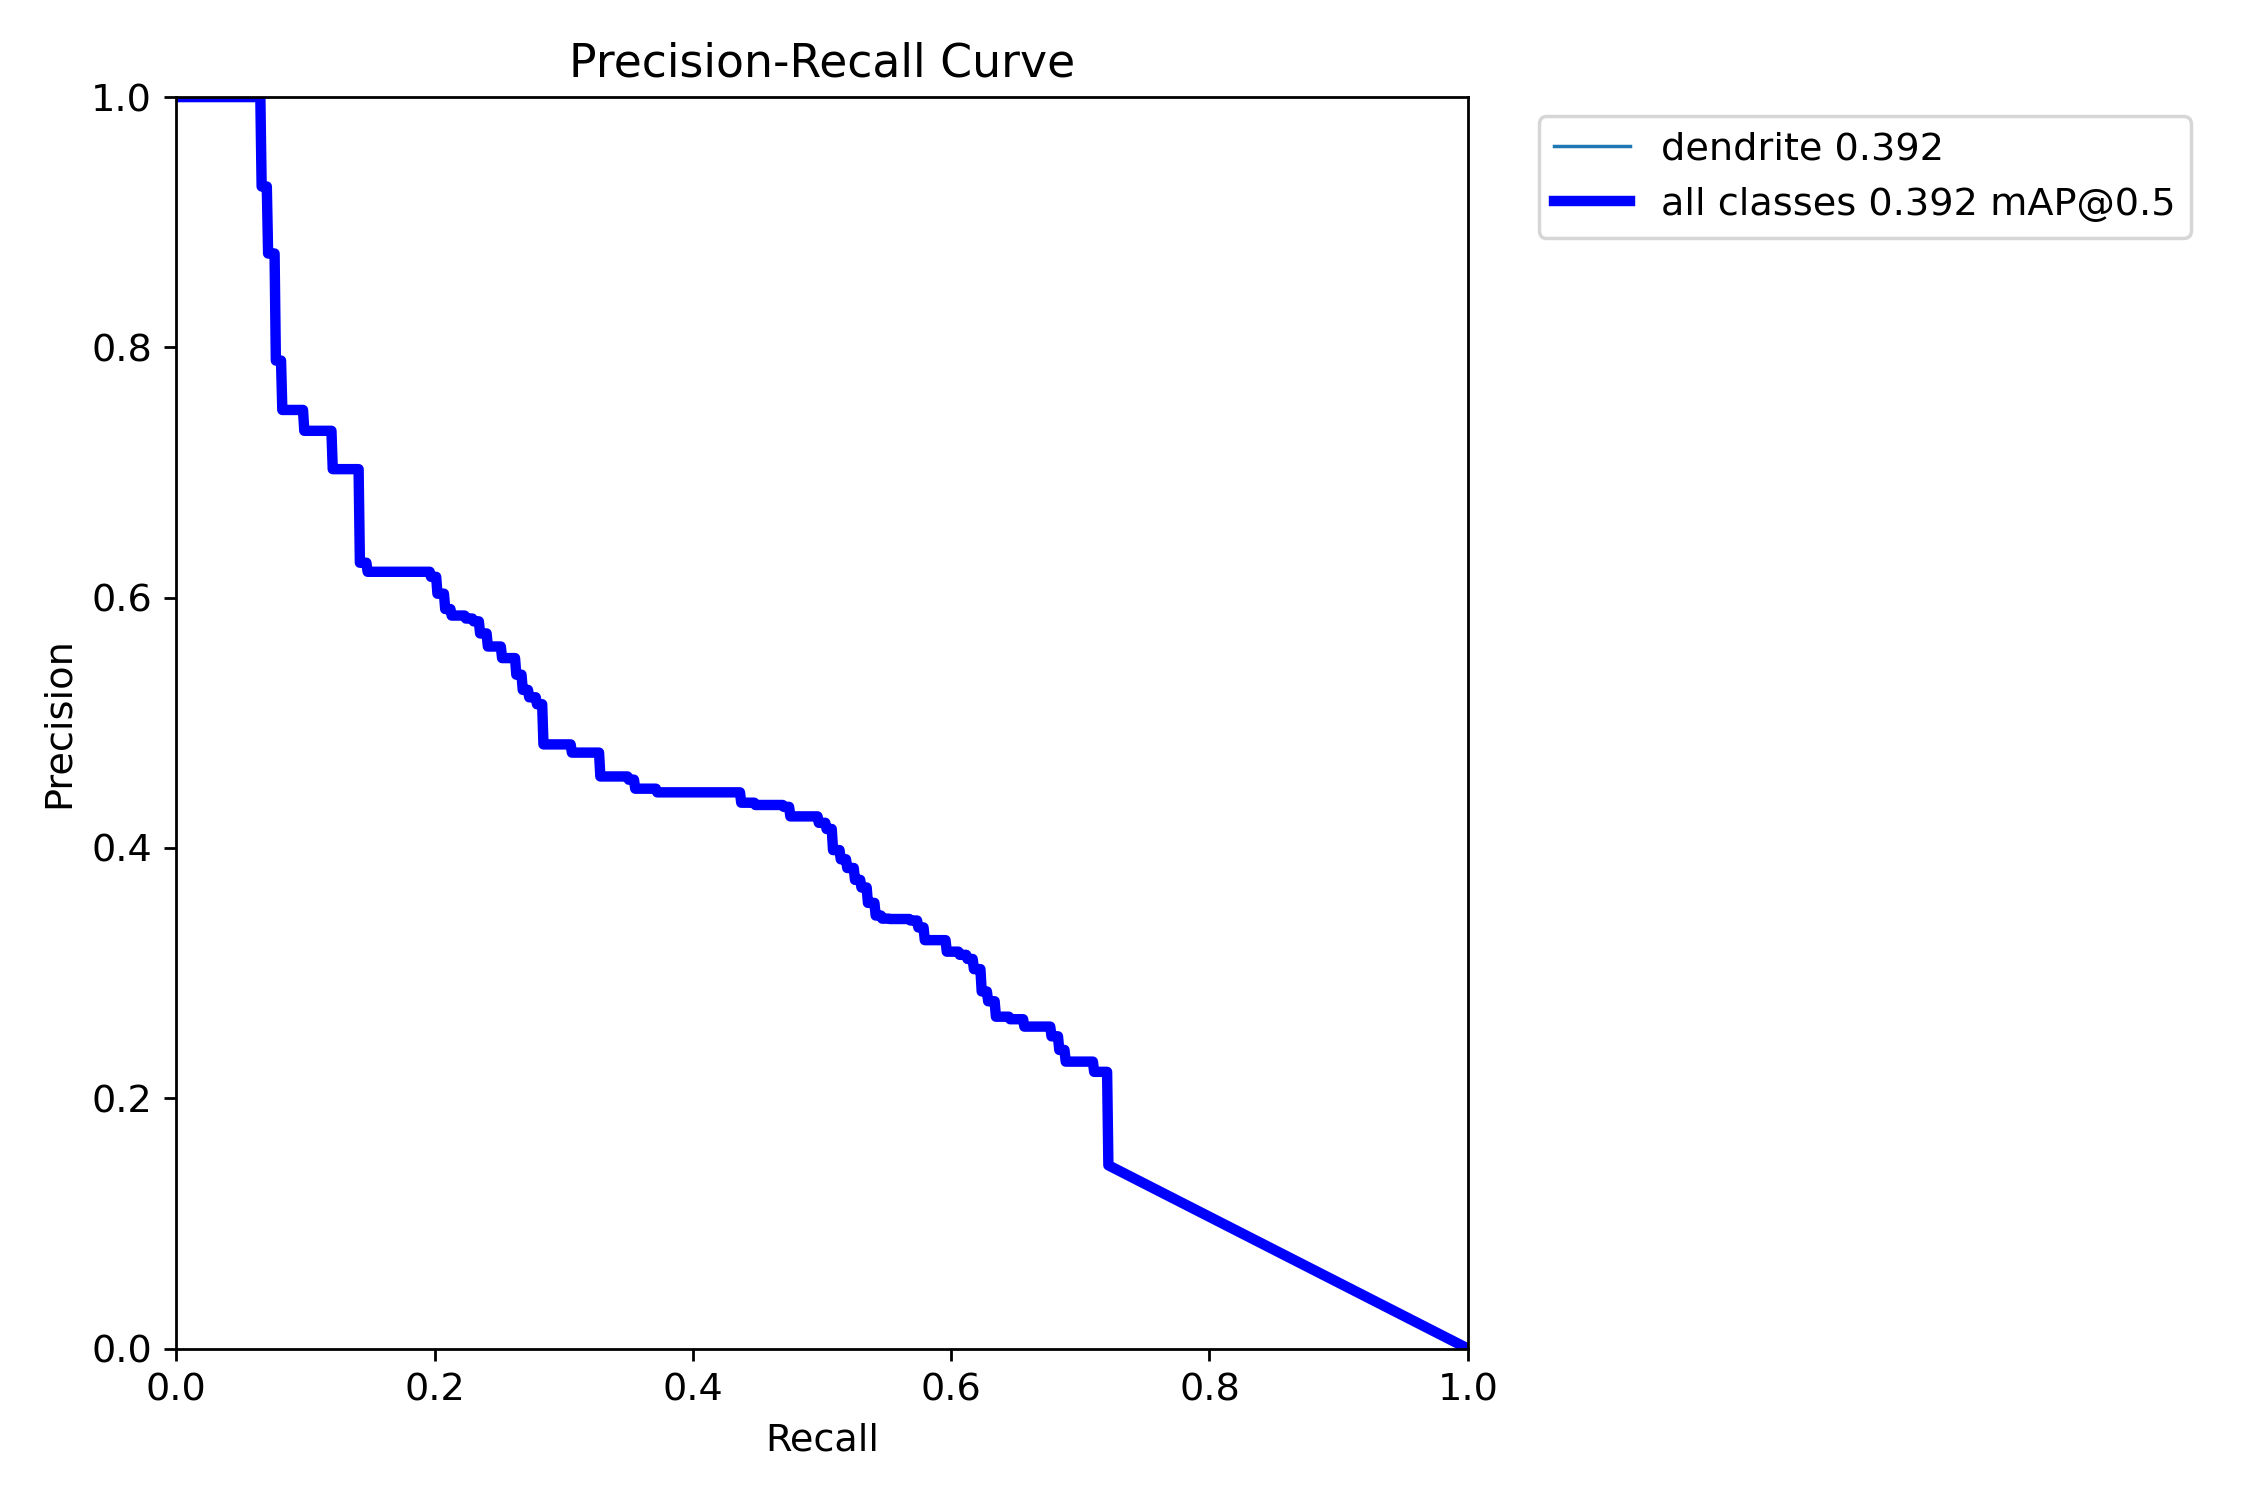
\includegraphics[width=0.92\linewidth]{assets/training/MaskPR_curve.png}
\caption{Mask precision-recall curve}
\end{figure}

\begin{figure}[H]
\centering
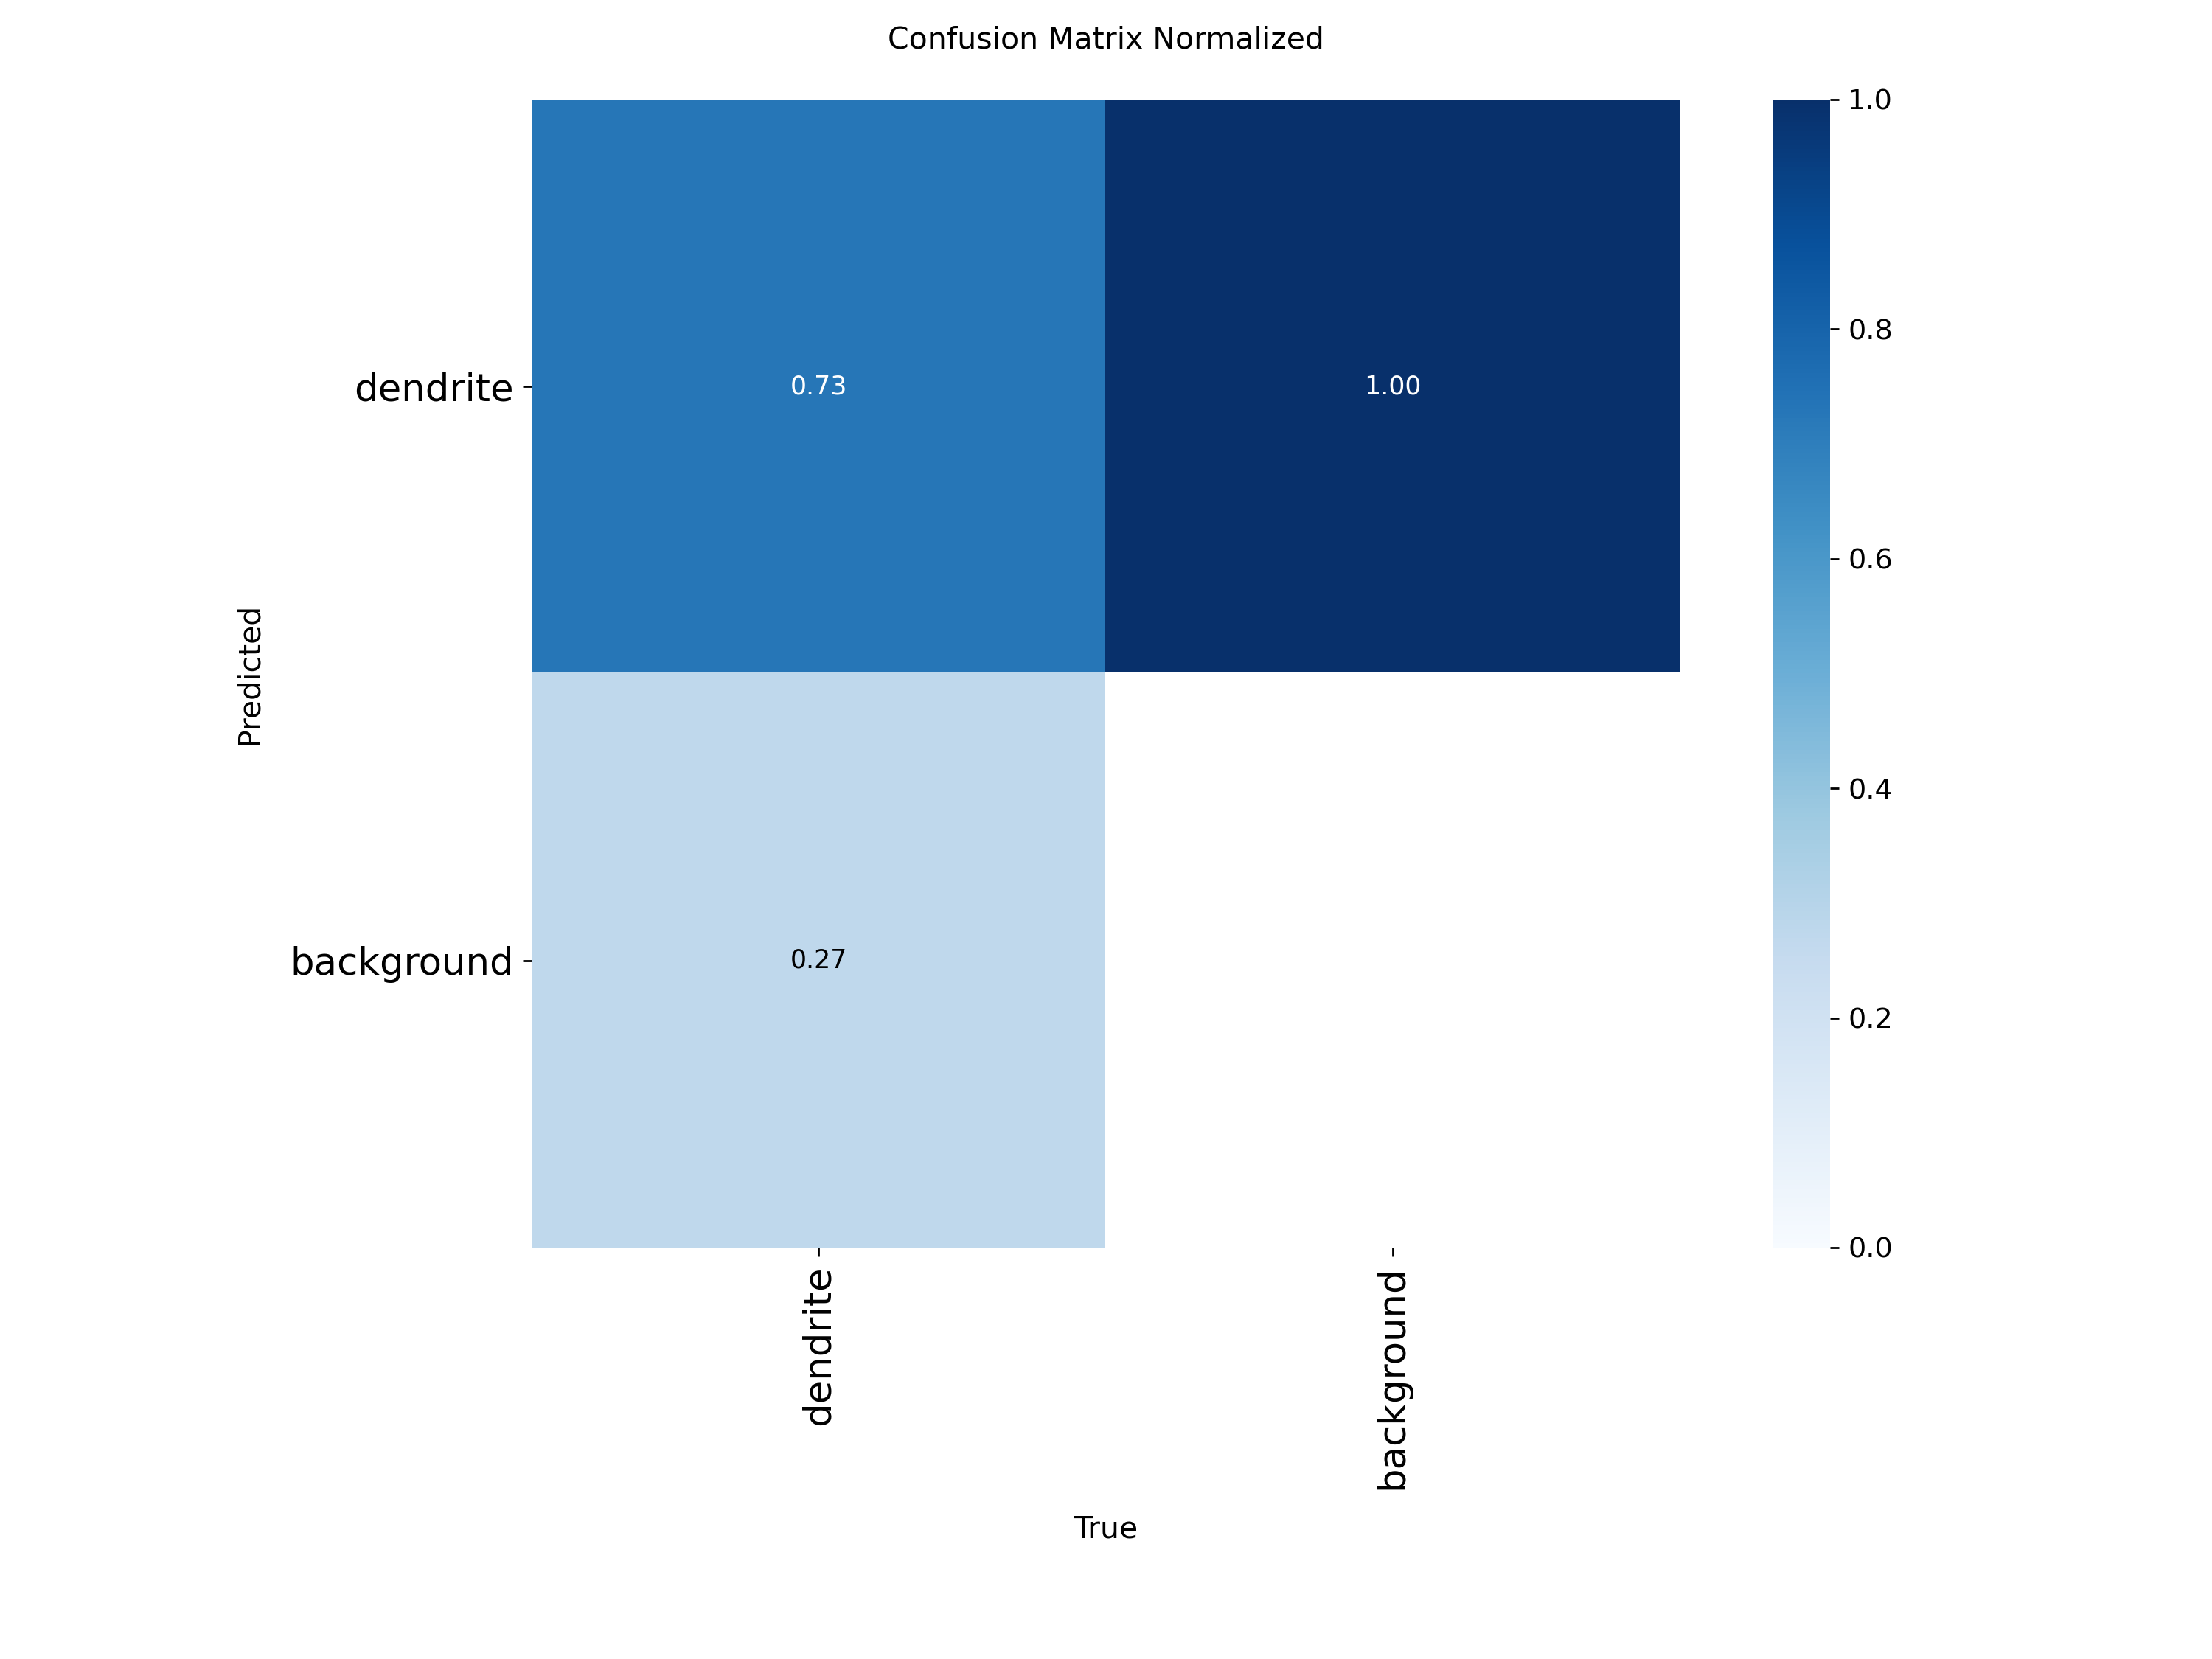
\includegraphics[width=0.92\linewidth]{assets/training/confusion_matrix_normalized.png}
\caption{Normalized confusion matrix}
\end{figure}

\section*{Conclusions}
The generated artifacts support the project submission requirements:
technical report format, quantitative metrics, comparison tables, and qualitative visual analysis.
Use this report as a reproducible baseline and regenerate it whenever new experiments are produced.

\end{document}
